\documentclass[11pt]{article}
\usepackage{geometry}
\geometry{a4paper, top=20mm, left=10mm, right=10mm, bottom=20mm}
\usepackage{graphicx}
\usepackage{amsmath,amssymb,amsthm}
\usepackage{amssymb}
\usepackage[utf8]{inputenc}
\usepackage{fancyhdr}
\usepackage{lastpage}
\usepackage{enumerate}
\usepackage{enumitem}
\usepackage{multicol}
\usepackage{subcaption}
\usepackage{ifthen}
\usepackage{listings}
\usepackage{color}
\usepackage{scalerel}
\usepackage{algorithmicx}
\usepackage[noend]{algpseudocode}
\usepackage[plain]{algorithm}
\usepackage{tikz}
\usetikzlibrary{er,positioning,shapes,arrows}
%------------------------------------------ preamble
%----- fancyhdr
\fancyhead[L]{Name: Maurice Wenig}
\fancyhead[R]{Matrikelnummer: 178049}
\fancyfoot{}
\rfoot{Seite \thepage\ von \pageref{LastPage}}
\pagestyle{fancy}
%----- aufgaben
\newtheoremstyle{break}{}{5mm}{}{}{\bfseries}{}{0mm}
{\textbf{\thmname{#1}\thmnumber{ #2:} \thmnote{\textit{#3}}\newline}}
\theoremstyle{break}
\newtheorem{task}{Aufgabe}
%----- new commands
\newcommand{\Romannumeral}[1]{\MakeUppercase{\romannumeral #1}}
\newcommand{\notiff}{\mathrel{{\ooalign{\hidewidth$\not\phantom{"}$\hidewidth\cr$\iff$}}}}
\newcommand{\set}[1]{\ensuremath{\{#1\}}}
\newcommand{\abs}[1]{\ensuremath{\left\vert #1 \right\vert}}
\newcommand{\norm}[1]{\ensuremath{\left\| #1 \right\|}}
\newcommand{\skal}[2]{\ensuremath{\left\langle #1 | #2 \right\rangle}}
\newcommand{\R}{\ensuremath{\mathbb{R}}}
\newcommand{\ndy}{
    \textcolor{red} {\hfill not done yet!}
    \reversemarginpar
    \marginpar{\raggedleft\textcolor{red}{\rule{2mm}{2mm}}}
}
%------------------------------------------ main
\begin{document}
%----- title
\begin{center}
\Large{Datenbanksysteme I}\\
\large{2. Übungsserie}
\end{center}
%----- tasks
\begin{task}
    \hfill\vspace{-5mm}
    \begin{enumerate}[label={(\alph*)}]
        \item[(a-c)] \hfill\vspace{-5mm}\\
        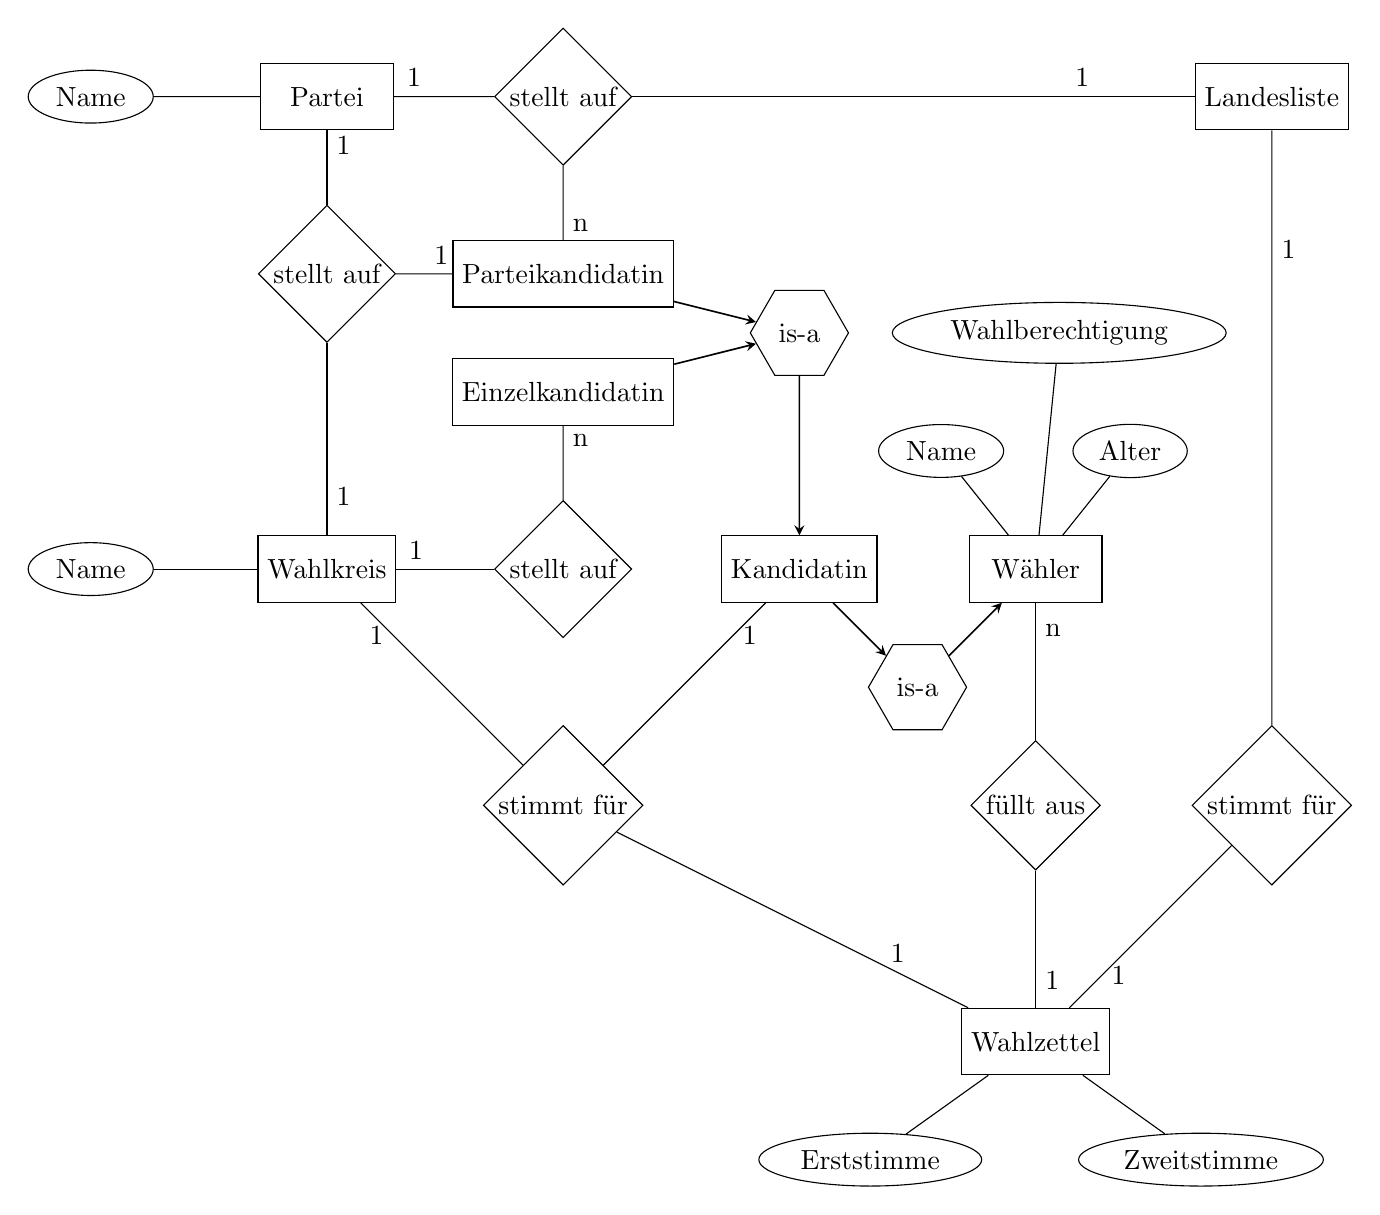
\begin{tikzpicture}[
                scale=3,
                isa/.style={regular polygon, regular polygon sides=6, draw=black!100}
            ]
            %\node[entity] (Wahlzettel)  at (0, 0) {Wahlzettel};
            %\node[attribute] (1) at (0, -4) {Erststimme};
            %\node[relationship] (fuellt) at (0, -2) {füllt aus};
            %\draw (Wahlzettel) -- (fuellt);
            %\draw (fuellt) -- (1);
            
            \node[entity] (Wahlkreis) at (0,0) {Wahlkreis};
            \node[entity] (Kandidat) at (2,0) {Kandidatin};
            \node[entity] (Kandidat_P) at (1,1.25) {Parteikandidatin};
            \node[entity] (Kandidat_E) at (1,0.75) {Einzelkandidatin};
            \node[entity] (Partei) at (0,2) {Partei};
            \node[entity] (Landesliste) at (4,2) {Landesliste};
            \node[entity] (Wahlzettel) at (3,-2) {Wahlzettel};
            \node[entity] (Waehler) at (3,0) {Wähler};

            \node[attribute] (Parteiname) at (-1, 2) {Name};
            \node[attribute] (Wahlkreisname) at (-1, 0) {Name};
            \node[attribute] (Waehlername) at (2.6, 0.5) {Name};
            \node[attribute] (Alter) at (3.4, 0.5) {Alter};
            \node[attribute] (Zeit) at (3.1, 1) {Wahlberechtigung};
            \node[attribute] (Erststimme) at (2.3, -2.5) {Erststimme};
            \node[attribute] (Zweitstimme) at (3.7, -2.5) {Zweitstimme};

            \node[isa] (Kandidat_isa) at (2,1) {is-a};
            \node[isa] (Waehler_isa) at (2.5,-0.5) {is-a};
    
            \node[relationship] (stimmt_fuer1) at (1,-1) {stimmt für};
            \node[relationship] (stimmt_fuer2) at (4,-1) {stimmt für};
            \node[relationship] (stellt_auf1) at (0,1.25) {stellt auf};
            \node[relationship] (stellt_auf2) at (1,2) {stellt auf};
            \node[relationship] (stellt_auf3) at (1,0) {stellt auf};
            \node[relationship] (fuellt_aus) at (3,-1) {füllt aus};

            \draw (Partei) -- (Parteiname);
            \draw (Wahlkreis) -- (Wahlkreisname);
            \draw (Waehler) -- (Waehlername);
            \draw (Waehler) -- (Alter);
            \draw (Waehler) -- (Zeit);
            \draw (Wahlzettel) -- (Erststimme);
            \draw (Wahlzettel) -- (Zweitstimme);

            \draw (Kandidat) edge[->, > = stealth, semithick] (Waehler_isa);
            \draw (Waehler_isa) edge[->, > = stealth, semithick] (Waehler);

            \draw (Kandidat_P) edge[->, > = stealth, semithick] (Kandidat_isa);
            \draw (Kandidat_E) edge[->, > = stealth, semithick] (Kandidat_isa);
            \draw (Kandidat_isa) edge[->, > = stealth, semithick] (Kandidat);
    
            \draw (Waehler) -- node[pos=0.2, right]{n} (fuellt_aus);
            \draw (Wahlzettel) -- node[pos=0.2, right]{1} (fuellt_aus);
    
            \draw (Wahlkreis) -- node[pos=0.2, left]{1} (stimmt_fuer1);
            \draw (Kandidat) -- node[pos=0.2, right]{1} (stimmt_fuer1);
            \draw (Wahlzettel) -- node[pos=0.2, above]{1} (stimmt_fuer1);
    
            \draw (Wahlzettel) -- node[pos=0.2, right]{1} (stimmt_fuer2);
            \draw (Landesliste) -- node[pos=0.2, right]{1} (stimmt_fuer2);
    
            \draw (Partei) -- node[pos=0.2, right]{1} (stellt_auf1);
            \draw (Kandidat_P) -- node[pos=0.2, above]{1} (stellt_auf1);
            \draw (Wahlkreis) -- node[pos=0.2, right]{1} (stellt_auf1);

            \draw (Landesliste) -- node[pos=0.2, above]{1} (stellt_auf2);
            \draw (Partei) -- node[pos=0.2, above]{1} (stellt_auf2);
            \draw (Kandidat_P) -- node[pos=0.2, right]{n} (stellt_auf2);

            \draw (Kandidat_E) -- node[pos=0.2, right]{n} (stellt_auf3);
            \draw (Wahlkreis) -- node[pos=0.2, above]{1} (stellt_auf3);
        \end{tikzpicture}
        \item[(d)] Nein, es wird z.B. nicht dargestellt, dass ein Wähler nur in seinem eigenen Wahlkreis abstimmen darf, da die Beziehung sich auf irgendein Element in der Menge der Wahlkreise bezieht und nicht auf ein spezifisches.
    \end{enumerate}
\end{task}

\begin{task}
    \hfill\vspace{-5mm}
    \begin{enumerate}[label={(\alph*)}]
        \item 3
        \item[(b,c)] $\text{Tutor}\times\text{Student}\rightarrow\text{Übung}$, Ein Tutor kann keine 2 Übungen beim selben Studenten haben\\
        $\text{Tutor}\times\text{Übung}\rightarrow\text{Student}$, Ein Tutor kann nur einen Studenten pro Übung haben\\
        $\text{Übung}\times\text{Student}\rightarrow\text{Tutor}$, Ein Student kann nur einen Tutor pro Übung haben
        \item[(d)] $\text{Tutor}\times\text{Student}\rightarrow\text{Übung}$\\
        $\text{Übung}\times\text{Student}\rightarrow\text{Tutor}$ 
    \end{enumerate}
\end{task}

\begin{task}
    \hfill\vspace{-5mm}
    \begin{enumerate}[label={(\alph*)}]
        \item[(a,b)] User(\underline{id}, name)\\
        follows(\underline{id\_follows, id\_followed})\\
        Tweet(\underline{tweet\_id}, date, text, user\_id)\\
        likes(\underline{user\_id, tweet\_id}, date)
        \item[(c)] date von write kann Tweet zugeordnet werden, da die beiden Relationen eh den gleichen Schlüssel haben und zu einer Relation verfeinert werden.\\
        date von likes kann nicht Tweet zugeordnet werden, da nicht mehrere Instanzen eines Attributes in ein Attribut geschrieben werden können (/sollten).
    \end{enumerate}
\end{task}
\end{document}